\begin{figure*}[t!]
\centering
\begin{subfigure}[b]{0.48\textwidth}
  \centering
  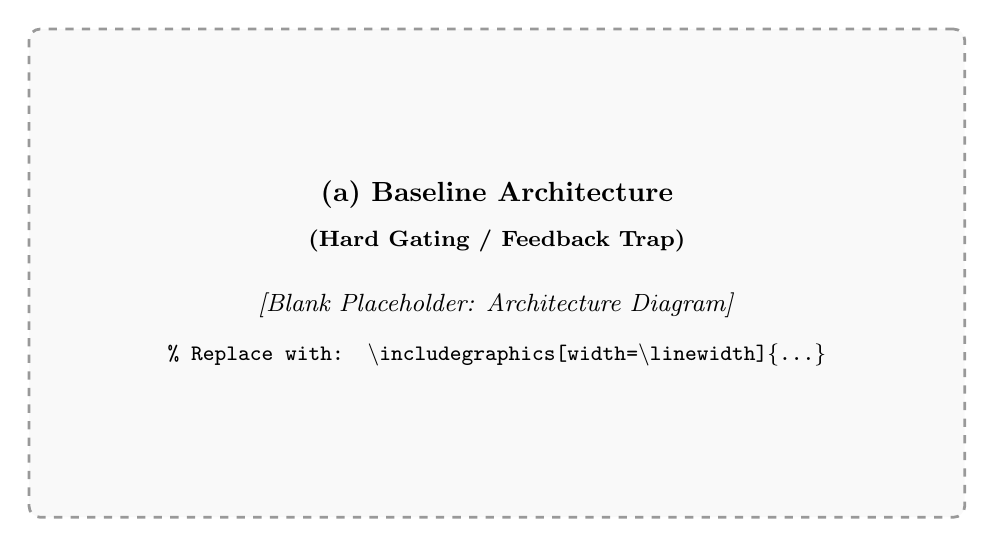
\begin{tikzpicture}
    \node[draw=black!40, dashed, fill=gray!5, rounded corners=4pt, line width=1pt, minimum width=0.98\linewidth, minimum height=6.2cm, align=center] {
      \textbf{\normalsize (a) Baseline Architecture}\\[1.5mm]
      \textbf{\footnotesize (Hard Gating / Feedback Trap)}\\[4mm]
      \textit{\small [Blank Placeholder: Architecture Diagram]}\\[2mm]
      {\footnotesize \texttt{\% Replace with: \textbackslash includegraphics[width=\textbackslash linewidth]\{...\}}}
    };
  \end{tikzpicture}
  \caption{Baseline Architecture}
  \label{fig:arch_baseline}
\end{subfigure}
\hfill
\begin{subfigure}[b]{0.48\textwidth}
  \centering
  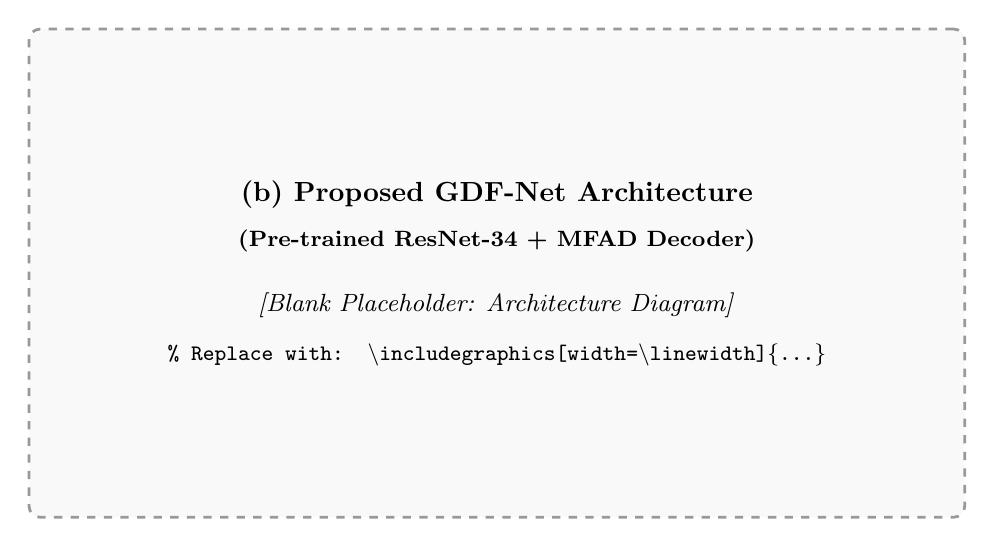
\begin{tikzpicture}
    \node[draw=black!40, dashed, fill=gray!5, rounded corners=4pt, line width=1pt, minimum width=0.98\linewidth, minimum height=6.2cm, align=center] {
      \textbf{\normalsize (b) Proposed GDF-Net Architecture}\\[1.5mm]
      \textbf{\footnotesize (Pre-trained ResNet-34 + MFAD Decoder)}\\[4mm]
      \textit{\small [Blank Placeholder: Architecture Diagram]}\\[2mm]
      {\footnotesize \texttt{\% Replace with: \textbackslash includegraphics[width=\textbackslash linewidth]\{...\}}}
    };
  \end{tikzpicture}
  \caption{Proposed GDF-Net Architecture (Ours)}
  \label{fig:arch_proposed}
\end{subfigure}
\caption{Architectural comparison between the coupled baseline and the proposed Gradient-Decoupled Feedback Network (\textbf{GDF-Net}). \textbf{(a) Baseline Architecture (Hard Gating / Feedback Trap):} Relies on a custom 4-stage convolutional encoder trained from scratch. The non-differentiable indicator gating ($\mathbb{I}(f_{\text{mask}} > 0.5)$) induces complete gradient paralysis ($\nabla_{f_{\text{mask}}} \equiv 0$), while unconstrained recursive backpropagation across feedback steps ($t=1 \to t=2$) injects past prediction errors into internal representations, triggering catastrophic Batch Normalization drift and irreversible false-positive expansion. \textbf{(b) Proposed GDF-Net Architecture (Ours):} Employs a pre-trained ResNet-34 transfer backbone accepting a 4-channel input stem, where the detached spatial prior ($m^{(t-1)}.\text{detach}()$) is adaptively modulated by a learned spatial gate. The Feedback Firewall strictly eliminates backward recursive gradient dependencies ($\nabla_{m^{(t-1)}} \equiv 0$), while the Multi-Scale Feedback Attention Decoder (\textbf{MFAD}) provides smooth, non-zero gradient modulation ($\mathbf{F} \odot (1.0 + \text{Att}(m))$) across all five hierarchical decoder scales, ensuring stable training convergence, robust false-positive suppression, and sharp anatomical boundary refinement.}
\label{fig:architecture}
\label{fig:architecture_diagram}
\end{figure*}
